\chapter{High Directional Link}

\section{Extra images}
\begin{figure}[htb]
    \centering
    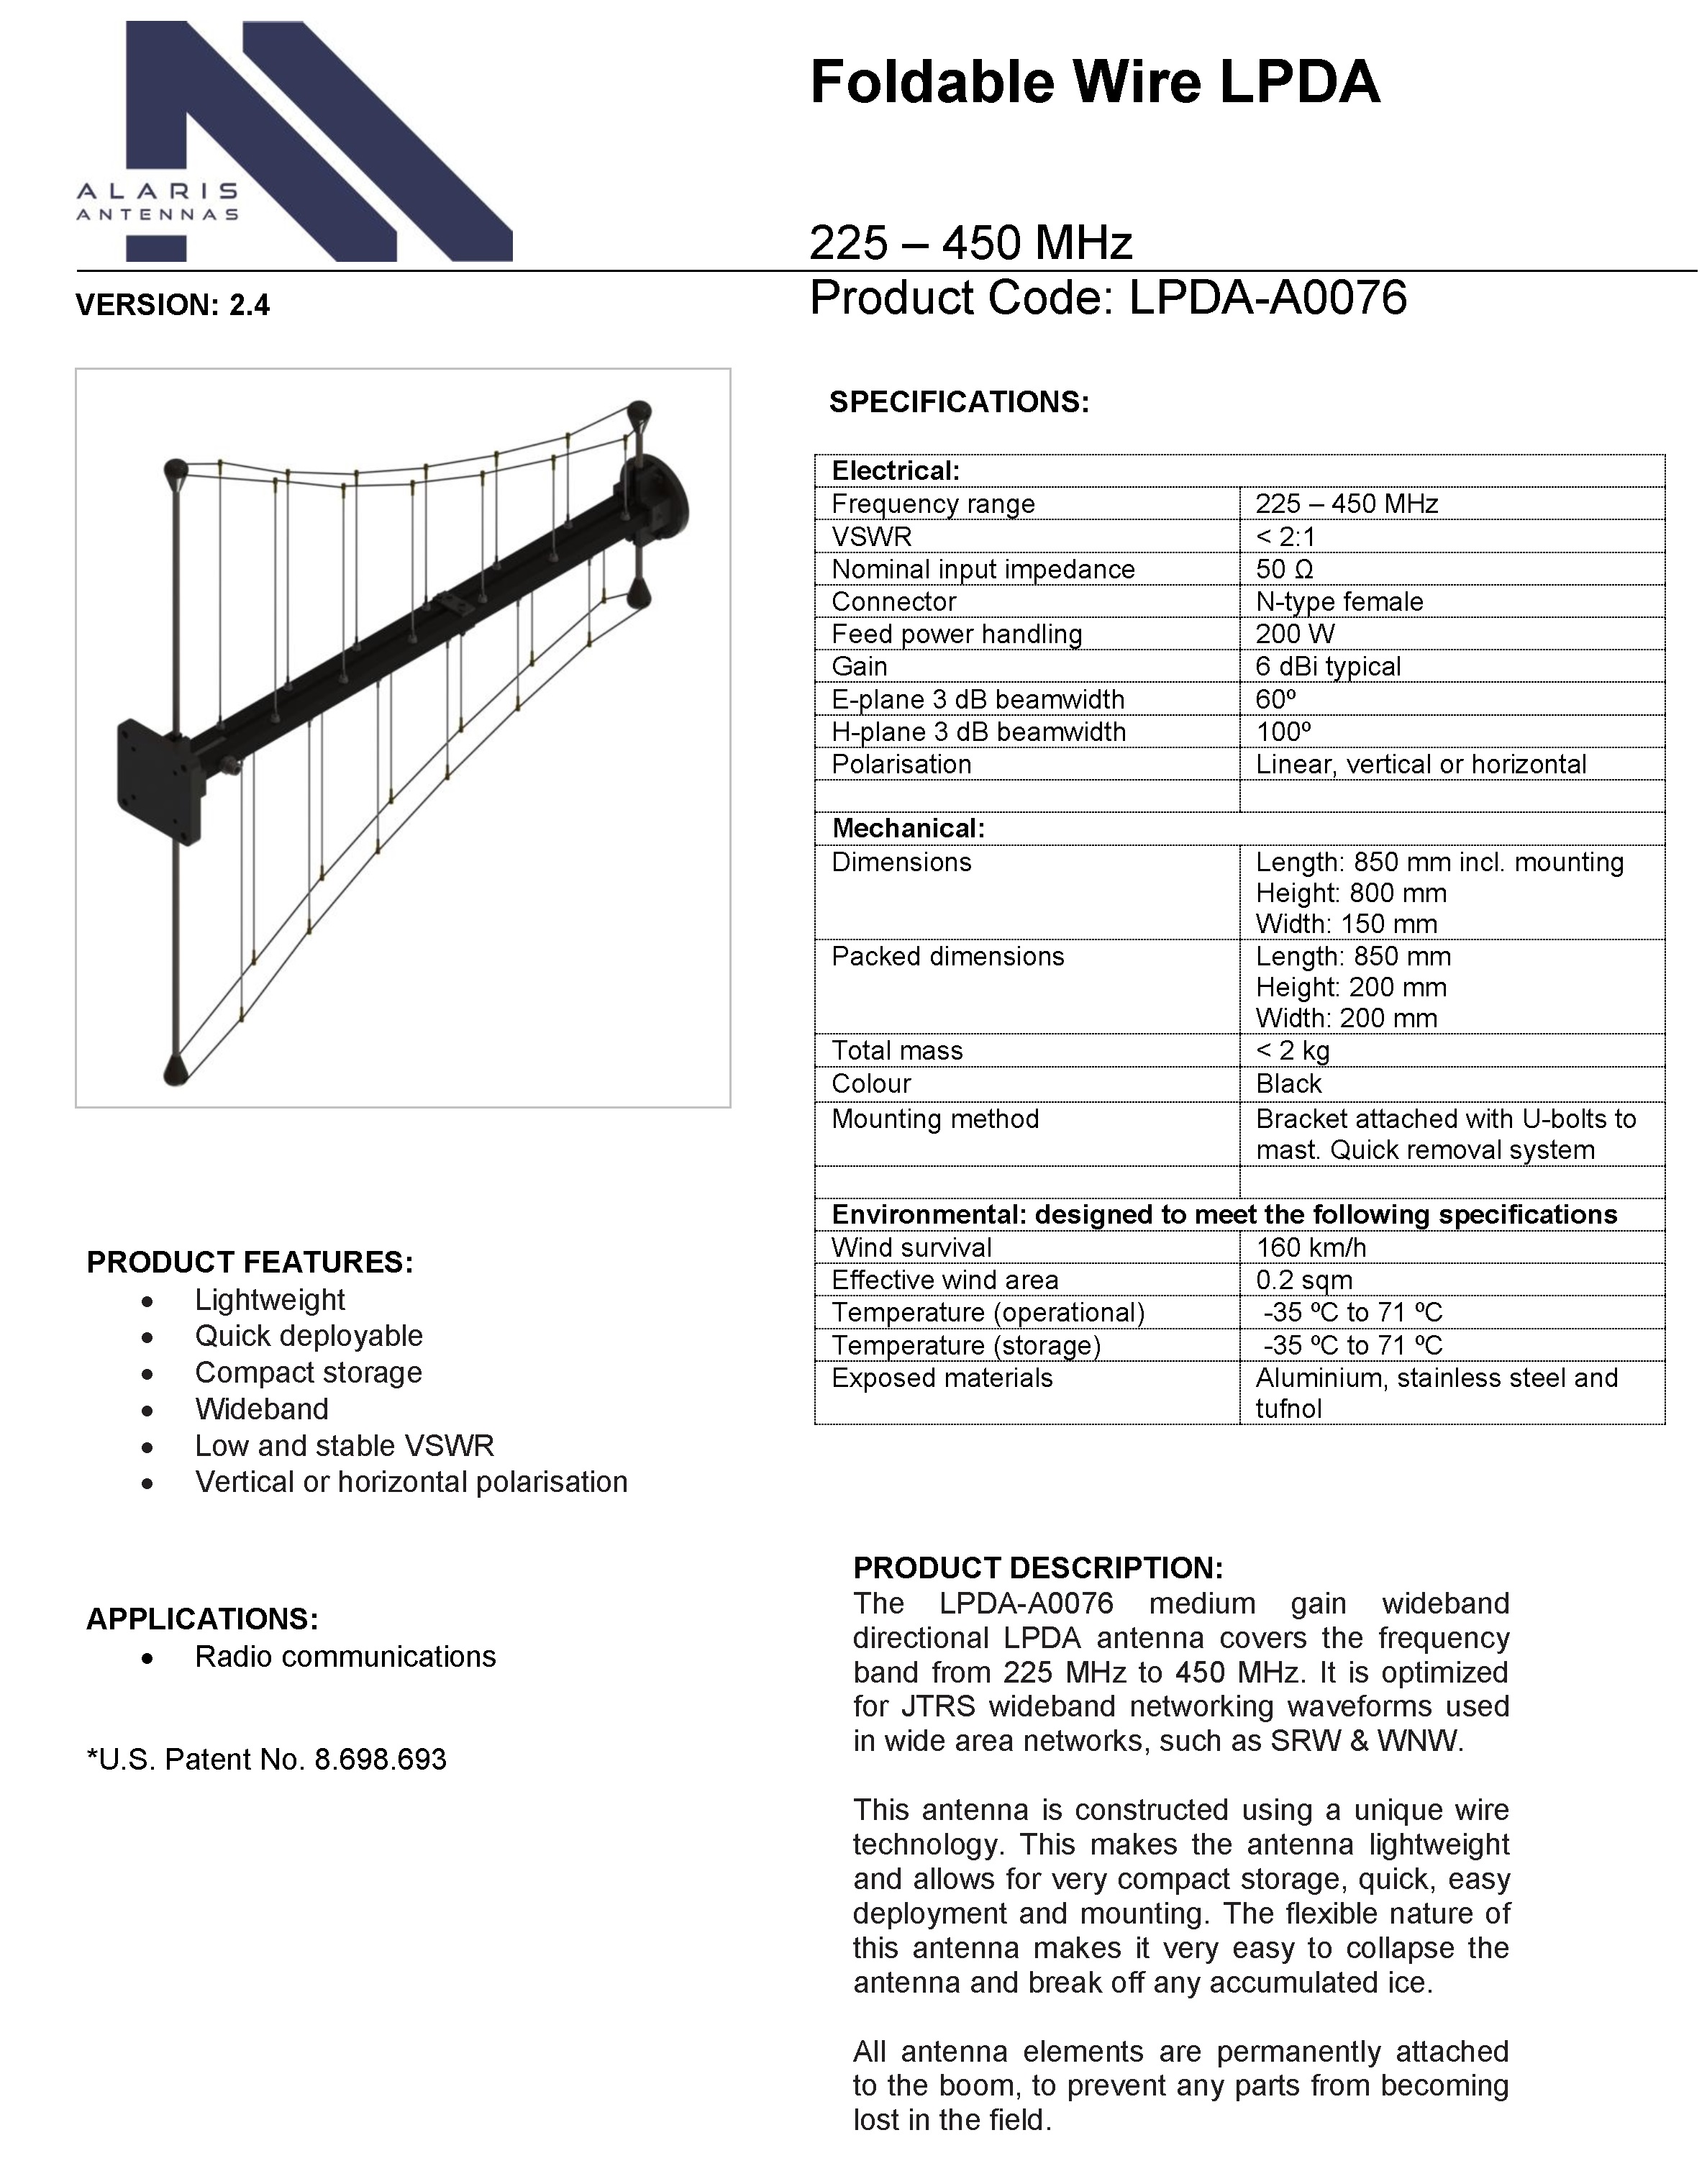
\includegraphics[width=1\textwidth]{figures/Yannis/LPDA.jpg}
    \caption{Foldable wire LPDA specifications by ALARIS antennas.}
    \label{LPDA1}
\end{figure}

\begin{figure}[htb]
    \centering
    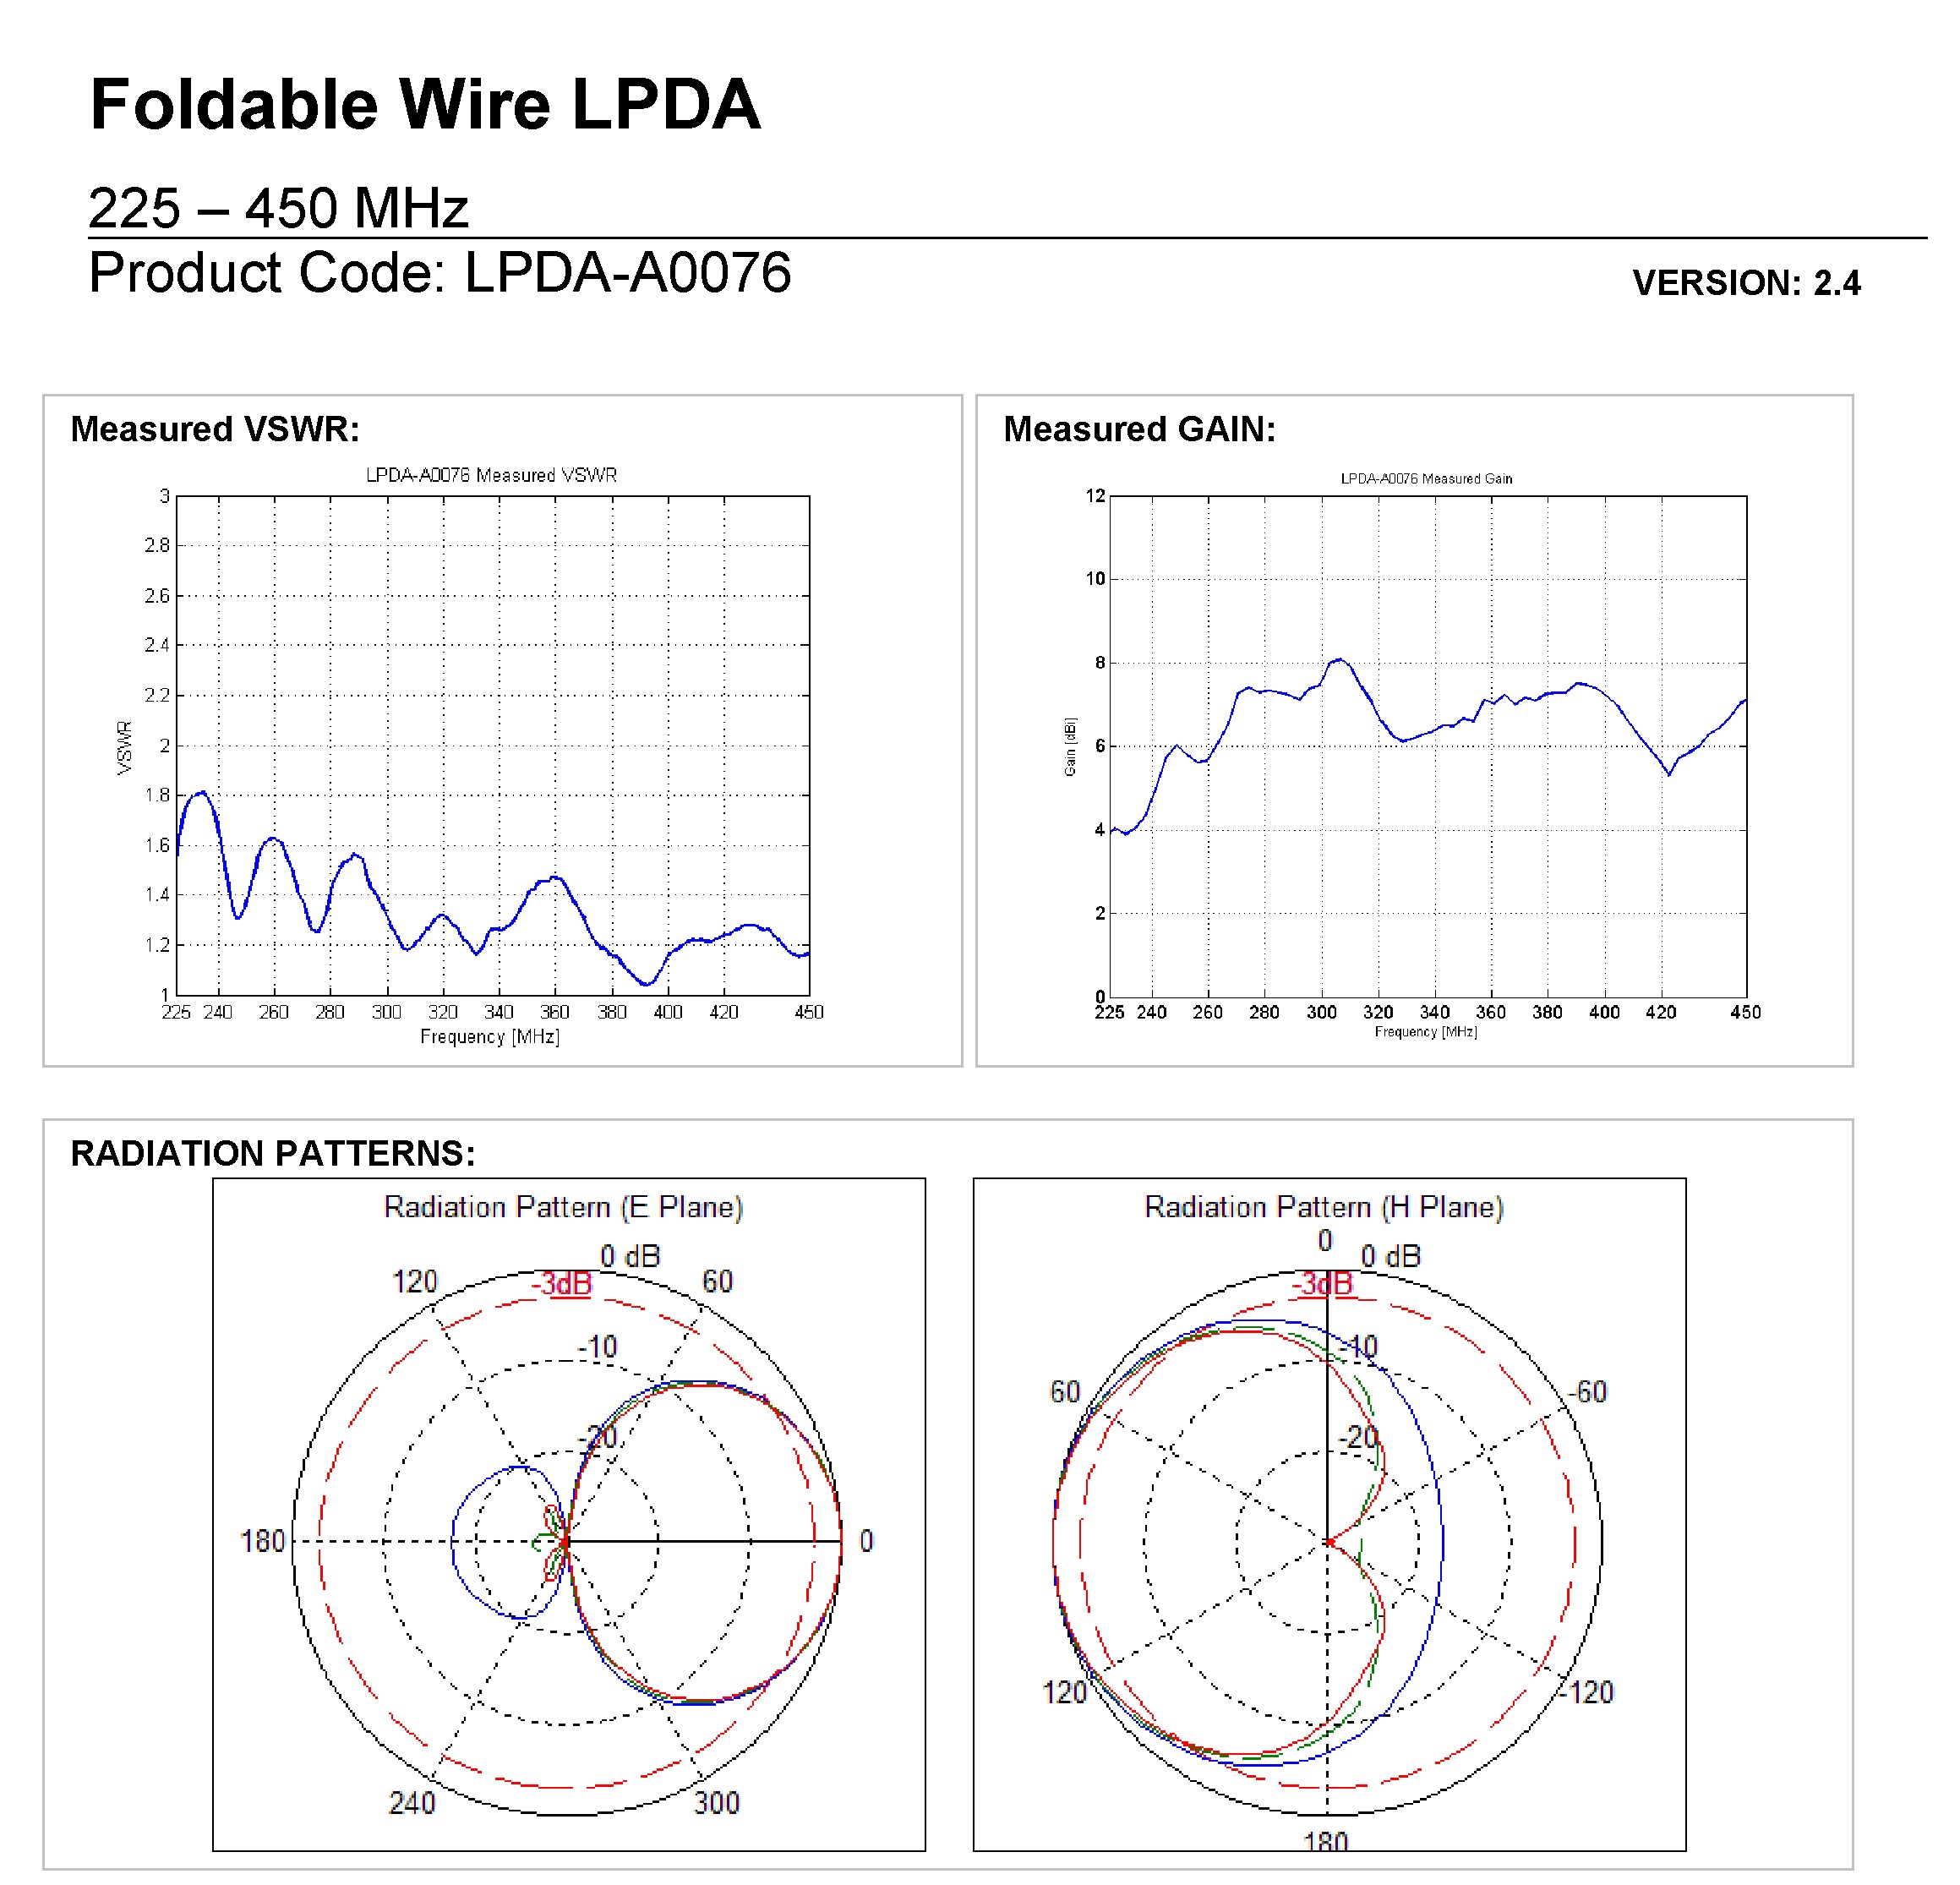
\includegraphics[width=1\textwidth]{figures/Yannis/lpda23.jpg}
    \caption{Foldable wire LPDA specifications by ALARIS antennas.}
    \label{LPDA2}
\end{figure}

\begin{table}[htb]
\centering
\begin{tabular}{| c | c | c | c | c | c | c | c |}
\hline
 f (MHz) & Gain (dBi) & HPBW & Length (mm) & $Gain_{array}$ & N & S & Diam \\ 
 \hline
 300 & 7.8 & 64.5$^\circ$ & 800 & 16.6 & 4 & 0.2 & 0.287 \\  
 \hline
 300 & 5.8 & 74.45$^\circ$ & 600 & 15.1 & 3 & 0.2 & 0.287 \\  
 \hline
 300 & 24.2 & 36.5$^\circ$ & 1160 & 19 & 4 & 0.29 & 0.42 \\
 \hline
 300 & 18.17 & 42.25$^\circ$ & 870 & 17.1 & 3 & 0.29 & 0.42  \\
 \hline
 340 & 23.6 & 37$^\circ$ & 1000 & 19 & 4 & 0.25 & 0.37  \\
 \hline
 340 & 17.7 & 42.8$^\circ$ & 750 & 19 & 3 & 0.25 & 0.37  \\
 \hline
 400 & 24.7 & 36.2$^\circ$ & 876 & 19.2 & 4 & 0.219 & 0.317  \\
 \hline
 400 & 18.5 & 41.8$^\circ$ & 657 & 17.2 & 3 & 0.219 & 0.317  \\
 \hline
\end{tabular}
\caption{Helical antenna design for different specifications. The "S" column corresponds to the spacing between turns and "Diam" column to the diameter of each loop.}
\label{table: Helicals}
\end{table}

\section{MATLAB code}
\label{matlab}

MATLAB code for LPDA design

\begin{lstlisting}
clear;
clc;
%% inputs
tau=0.9;
sigma=0.07;
f_high=400;
f_low=300;
B=f_high/f_low;% desired BW, ratio of limit freqs.
c=3*1e8;
%%
a=atand((1-tau)/(4*sigma));
B_ar=1.1+7.7*(1-tau)^2*cotd(a);
B_s=B_ar*B;
lambda_max=c/(f_low*1e6);
L=lambda_max*cotd(a)*(1-(1/B_s))/4
N=1+(log(B_s))/(log(1/tau))
sigmaZ=sigma/sqrt(tau);
lmax=lambda_max/2; % in meters
dmax=0.019; % outside diameter of elements in meters
ratio=lmax/dmax;
Za=120*(log(ratio)-2.25)
\end{lstlisting}

MATLAB code for helical antenna design.

\begin{lstlisting}
clear;
clc;
%% Input - Mechanical Parameters
f=400*1e6; % Hz
c=3*1e8; % speed of light
l=c/f; % wavelength in meters
N=3; % number of turns
a=0.00332/2; % radius of conductor
Diam=0.317; % diamter 
S=0.219; % gap between turns 
C=pi*Diam; % circomference of single turn
C_l=C/l;
%% 
alpha=atand(S/C); % pitch angle
L0=sqrt(S^2+C^2); % length of one turn
Length=N*S; % overall length
Wire_L=N*L0; % wire length
R=l*3/4; % 
backplane=pi*(R/2)^2; % reflector emv
if alpha<12 || alpha>14 
    fprintf('alpha smaller than 12 or larger than 14, %d',alpha)
elseif C/l<=3/4 || C/l>=4/3 
    fprintf('C/l problem, %d', C/l)
elseif N<3
    fprintf('N smaller or equal 3, %d', N)
else
    Zin=140*(C/l); % real part of input impedance, accuracy 20%
    HPBW=(52*(l^(3/2)))/(C*sqrt(N*S)); % Half power BW in degrees
    D=12*N*C^2*S/(l^3); % (max) directivity
    AR=(2*N+1)/(2*N); % Axial ratio
end
k1=0.8;
L=k1*(l+(l/(2*N))+S);

%% Array of 4
square=(1.5*l+R); % backplane emv
dis=1.5*l; % distance between array elements
elem_no=4; % element numbers
k=2*pi/l; % wavenumber

D_array2=elem_no*(1+Length/dis)*(dis/l);
D_HW=1.805*(elem_no*(1+Length/dis)*(dis/l)); % Hansen-Woodyard directivity
fprintf('\nTotal length %d meters', Length)
fprintf('\nTotal size of backplane %d meters', square)
fprintf('\nHPBW= %d degrees', HPBW)
fprintf('\nDirectivity of one %d dBi', D)
fprintf('\nDirectivity after HW %d dBi\n', D_HW)
\end{lstlisting}

MATLAB code for parabolic antenna design.

\begin{lstlisting}

clear;
clc;
%% inputs
f=400*1e6; % MHz
c=3*1e8; % speed of light
l=c/f; % wavelength in meters
eff=0.66; % efficiency factor 50-75%
D=0.9; % diameter in meters.

Gain=10*log10(eff*(pi*D/l)^2) % gain in dBi
HPBW=60*l/D % in degrees
\end{lstlisting}
